\documentclass[a4paper, 12pt]{article}%тип документа

%отступы
\usepackage[left=2cm,right=2cm,top=2cm,bottom=3cm,bindingoffset=0cm]{geometry}

%Русский язык
\usepackage[T2A]{fontenc} %кодировка
\usepackage[utf8]{inputenc} %кодировка исходного кода
\usepackage[english,russian]{babel} %локализация и переносы

%Вставка картинок
\usepackage{graphicx}
\graphicspath{{pictures/}}
\DeclareGraphicsExtensions{.pdf,.png,.jpg}

%Графики
\usepackage{multirow}
\usepackage{pgfplots}
\pgfplotsset{compat=1.9}

%Римские цифры
\newcommand{\RNumb}[1]{\uppercase\expandafter{\romannumeral #1\relax}}

%Математика
\usepackage{amsmath, amsfonts, amssymb, amsthm, mathtools}

%Заголовок
\author{Богданов Александр \\
	Б05-003}
\title{\textbf{Работа 5.1.3 \\ 
		Изучение рассеяния медленных электронов на атомах (эффект Рамзауэра)}}

\begin{document}

\maketitle

\textbf{Цель работы:} исследовать энергетическую зависимость вероятности рассеяния электронов атомами,  определить энергию электронов,  при которой наблюдается <<просветление>> ксенона,  и оценить размер его внешней электронной оболочки.

\textbf{В работе используются:} Тиратрон ТГ3-01/1.3Б,  заполненный инертным газом,  блок источников питания, вольтметры В7-22А (В7-58),  осциллограф С1-83.
\\

\textbf{Теоретические положения:}\\\par

	Эффект Рамзауэра -- явление аномально слабого рассеяния медленных электронов атомами инертных газов. 

	Эффективное сечение реакции --  величина,  характеризующая вероятность перехода системы двух сталкивающихся частиц в результате их рассеяния  в определенное конечное состояние.  Сечение $\sigma$ равно отношению числа $N$ таких переходов в единицу времени к плотности $nv$ потока рассеиваемых частиц, падающих на мишень, т.е. к числу частиц, проходящих в единицу времени через единичную площадку, перпендикулярную к их скорости $v$.

\[ \sigma = \dfrac{N}{nv}\]

	Таким образом, сечение имеет размерность площади. Качественная картина результатов измерения упругого рассеяния электронов в аргоне:

	\begin{figure}[h!]
		\centering
		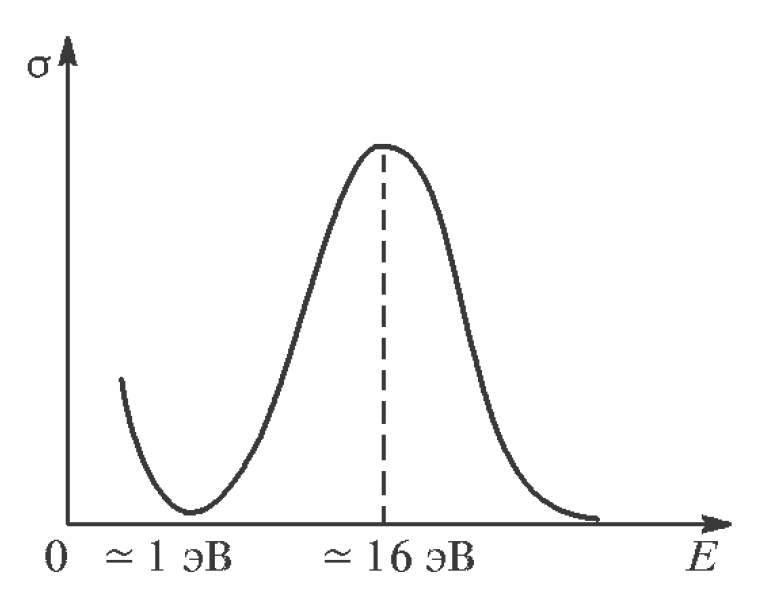
\includegraphics[scale=0.3]{График_1.PNG}
	\end{figure}

	По мере уменьшения энергии электрона от нескольких десятков электрон-вольт поперечное сечение его упругого рассеяния растет,  как это и следует из очень простых рассуждений: чем меньше скорость электрона,  тем медленнее он <<проскакивает>> мимо атома,  тем больше время взаимодействия электронов с атомом и, тем самым, больше вероятность этого взаимодействия, т.е. сечение реакции. Однако в эксперименте наблюдалось, что при энергиях меньше 16 эВ сечение начинает уменьшаться,  а при $E \simeq 1$ эВ практически равно нулю,  т.е. аргон становится прозрачным для электронов.  При дальнейшем уменьшении энергии электронов сечение рассеяния опять начинает возрастать.

	С точки зрения квантовой теории картина рассения выглядит иначе.  Внутри атома потенциальная энергия налетающего электрона $U$ отлична от нуля,  скорость электрона изменяется,  становясь равной $v'$ в соответствие с законом сохранения энергии,  а значит,  изменяется и длина его волны де Бройля.  Таким образом,  по отношению к электронной волне атом ведет себя как преломляющая среда с относительным показателем преломления:
	
\[ n = \dfrac{\lambda}{\lambda'} = \sqrt{1 - \dfrac{U}{E}} \]

	Рассмотрим достаточно грубую модель: будем считать, что электрон рассеивается на одномерной потенциальной яме конечной глубины:

	\begin{figure}[h!]
		\centering
		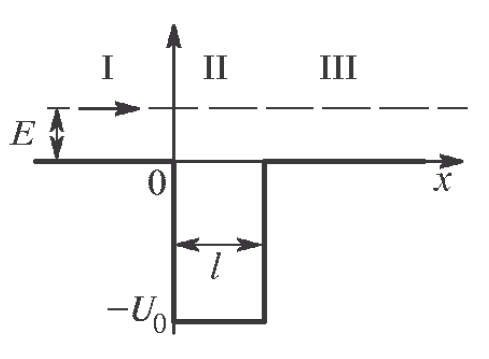
\includegraphics[scale=0.4]{Схема_1.PNG}
	\end{figure}

Уравнение Шредингера в данном случае имеет вид:

\begin{align}
	\psi'' + k^2 \psi = 0, \text{ где } k^2 = 
		\begin{cases}
			k_1^2 = \frac{2mE}{\hbar^2} & \text{~--- в областях I и III} \\
			k_2^2 = \frac{2m(E + U_0)}{\hbar^2} & \text{~--- в области II}
		\end{cases} 
\end{align}

	Коэффициент прохождения равен отношению квадратов амплитуд прошедшей и падающей волн, определяется выражением:
	
\[ D = \dfrac{16 k_1^2 k_2^2}{16 k_1^2 k_2^2 + 4(k_1^2 - k_2^2)^2 \sin^2(k_2l)}\]

	Максимален при условии:

\[k_2 l = \sqrt{\frac{2m(E_n + U_0)}{\hbar^2}}l = n \pi, \ n = 1, 2, 3, \ldots\]

	Это условие легко получить,  рассматривая интерференцию волн де Бройля в атоме.  Движущемуся электрону соответствует волна де Бройля,  длина которой определяется соотношением $\lambda = h / mv$.  Если кинетическая энергия электрона невелика,  то $E = mv^2 / 2$ и $\lambda = h / \sqrt{2mE}$.  При движении электрона через атом длина волны де Бройля становится меньше и равна $\lambda' = h / \sqrt{2m(E + U_0)}$,  где $U_0$ -- глубина атомного потенциала.  При этом волна де Бройля отражается от границ атомного потенциала, т.е. от поверхности атома,  и происходит интерференция прошедшей через атом волны 1 и волны 2, о траженной от передней и задней границы атома (эти волны когерентны):

	\begin{figure}[h!]
		\centering
		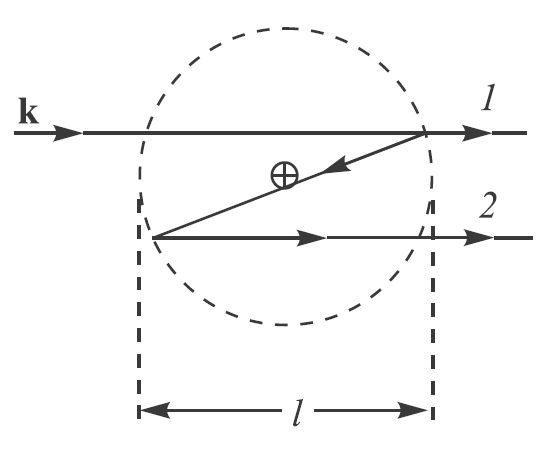
\includegraphics[scale=0.4]{Схема_2.PNG}
	\end{figure}

	Условие первого интерференционного максимума:

\[2l = \dfrac{h}{\sqrt{2m(E_1 + U_0)}}\]

Условие первого интерференционного минимума:

\[2l = \dfrac{3}{2}\dfrac{h}{\sqrt{2m(E_2 + U_0)}}\]

Эффективный размер атома:

\[l = \dfrac{h\sqrt{5}}{\sqrt{32m(E_2 - E_1)}}\]

Эффективная глубина потенциальной ямы атома:

\[U_0 = \dfrac{4}{5}E_2 - \dfrac{9}{5}E_1\]

\textbf{Экспериментальная установка:}\\\par

	\begin{figure}[h!]
		\centering
		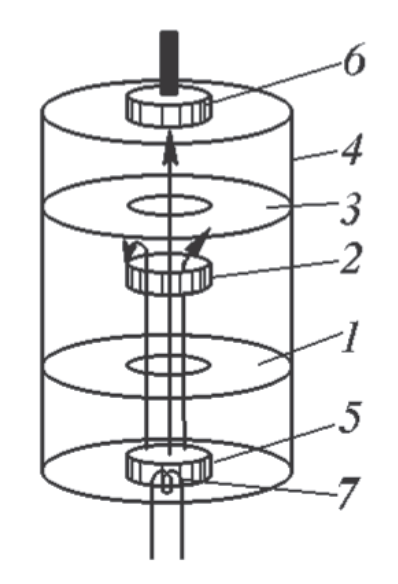
\includegraphics[scale=0.4]{Схема_3.PNG}
	\end{figure}

	Тиратрон: 1, 2, 3 -- сетки; 4 -- внешний металлический цилиндр; 5 -- катод; 6 -- анод; 7 -- накаливаемая спираль.

	В данной работе для изучения эффекта Рамзауэра используется тиратрон ТГ3-01/1.3Б, заполненный инертным газом.  Электроны эмитируются катодом, ускоряются напряжением $V$ и рассеиваются на атомах газа.  Сетки соединены между собой и имеют один потенциал,  примерно равный потенциалу анода. Рассеянные электроны отклоняются и уходят на сетку, а оставшиеся достигают анода, создавая ток $I_{\text{а}}$.  Таким образом,  поток электронов на расстоянии $x$ от ускоряющей сетки уменьшается с ростом $x$.  ВАХ анода,  согласно теории, должна соответствовать:

\[I_{\text{а}} = I_0 e^{-Cw(V)}, \ C = L n_{\text{а}} \Delta_{\text{а}},\]

	где $I_0 = eN_0$ -- ток катода,  $I_{\text{а}} = eN_{\text{а}}$ -- анодный ток,  $L$~--- расстояние между катодом и анодом,  $\Delta_{\text{а}}$ -- площадь поперечного сечения атома,  $n_{\text{а}}$ -- концентрация газа в лампе,  $w(V)$ -- вероятность рассеяния на атоме.  При этом по измеренной ВАХ тиратрона можно определить зависимость вероятности рассеяния электрона от его энергии из соотношения:

\[w(V) = - \dfrac{1}{C}\ln{\dfrac{I_{\text{а}}(V)}{I_0}}\]

	Схема экспериментальной установки конструктивно осуществлена следующим образом: лампа-тиратрон расположена непосредственно на корпусе блока источников питания (БИП),  напряжение к электродам лампы подается от источников питания,  находящихся в корпусе прибора.  Регулировка напряжения и выбор режима работы установки производится при помощи ручек управления,  выведенных на лицевую панель БИП.

	\begin{figure}[h!]
		\centering
		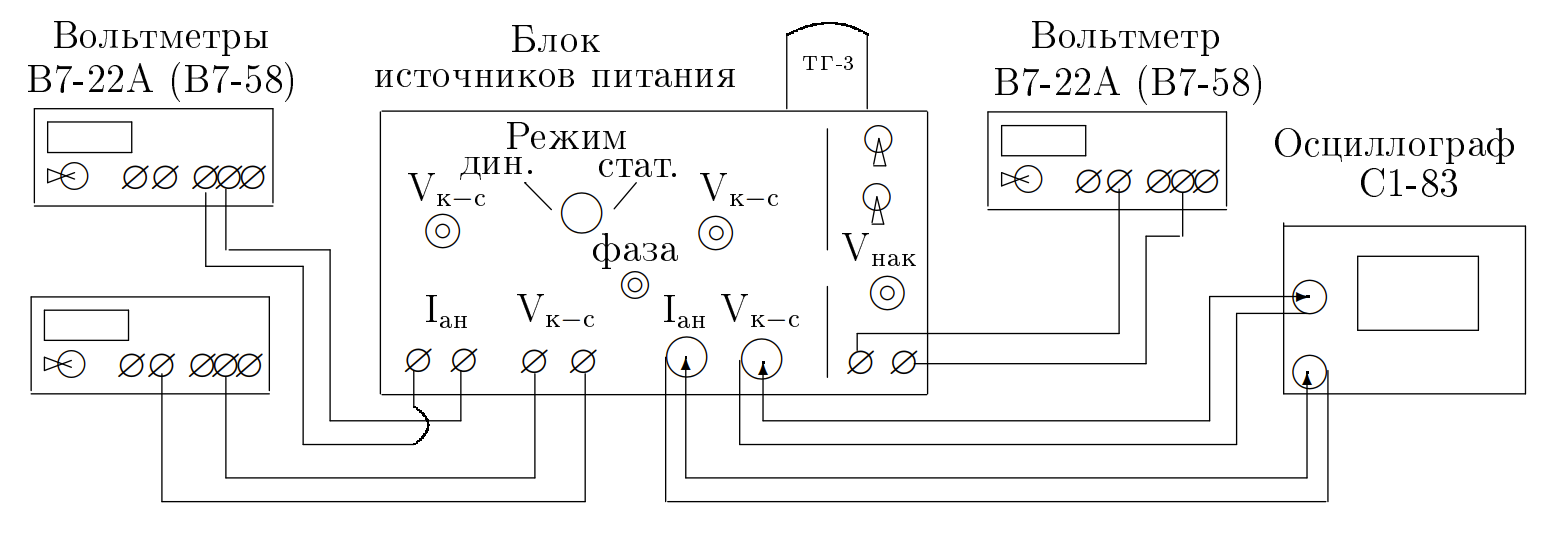
\includegraphics[scale=0.4]{Схема_4.PNG}
	\end{figure}
	
\textbf{Ход работы:}\\\par

\textbf{Вольт-амперная характеристика на экране осциллографа}

\begin{enumerate}

\item При максимальном ускоряющем напряжении измерим напряжение между катодом и сеткой,  соответствующие первому максимуму и минимуму,  а также напряжение пробоя:

	\begin{figure}[h!]
		\centering
		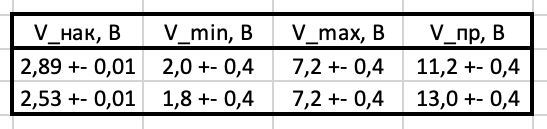
\includegraphics[scale=1]{Таблица_1.PNG}
	\end{figure}

\item Полученные на осциллографе ВАХ:

	\begin{figure}[h!]
		\centering
		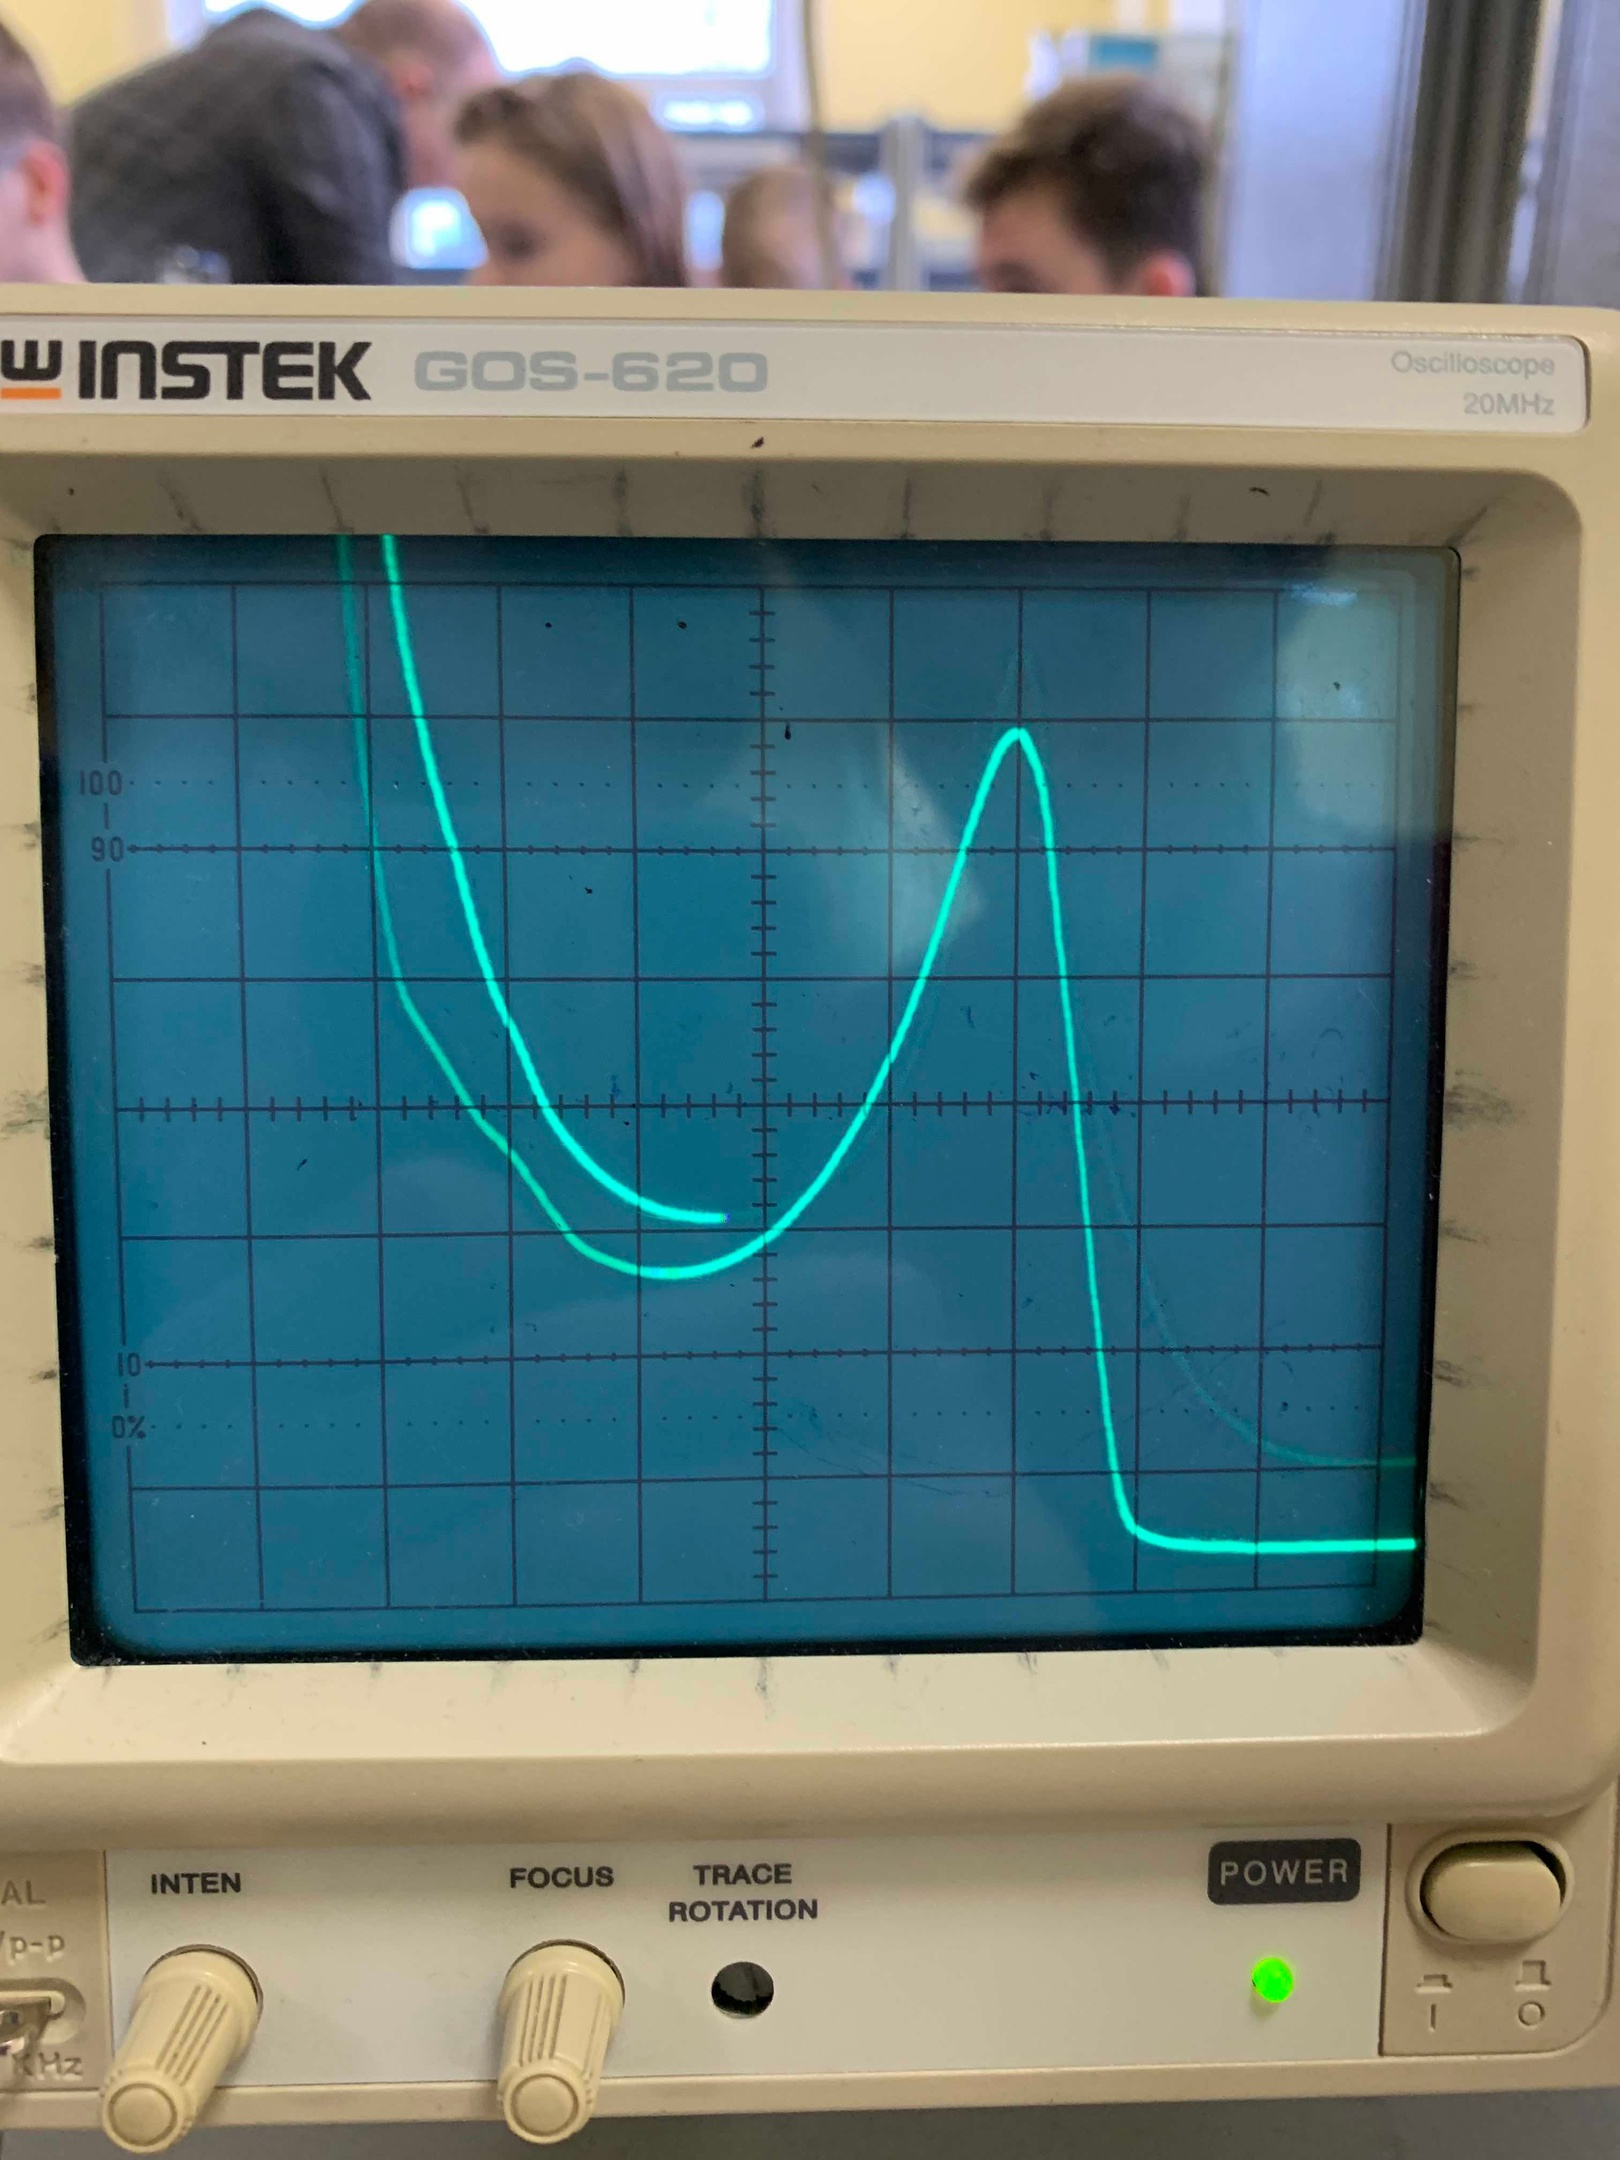
\includegraphics[scale=0.13]{Фото_1.PNG}
		\caption{$V_{\text{нак}} = 2.886$ В}
	\end{figure}
	
	\begin{figure}[h!]
		\centering
		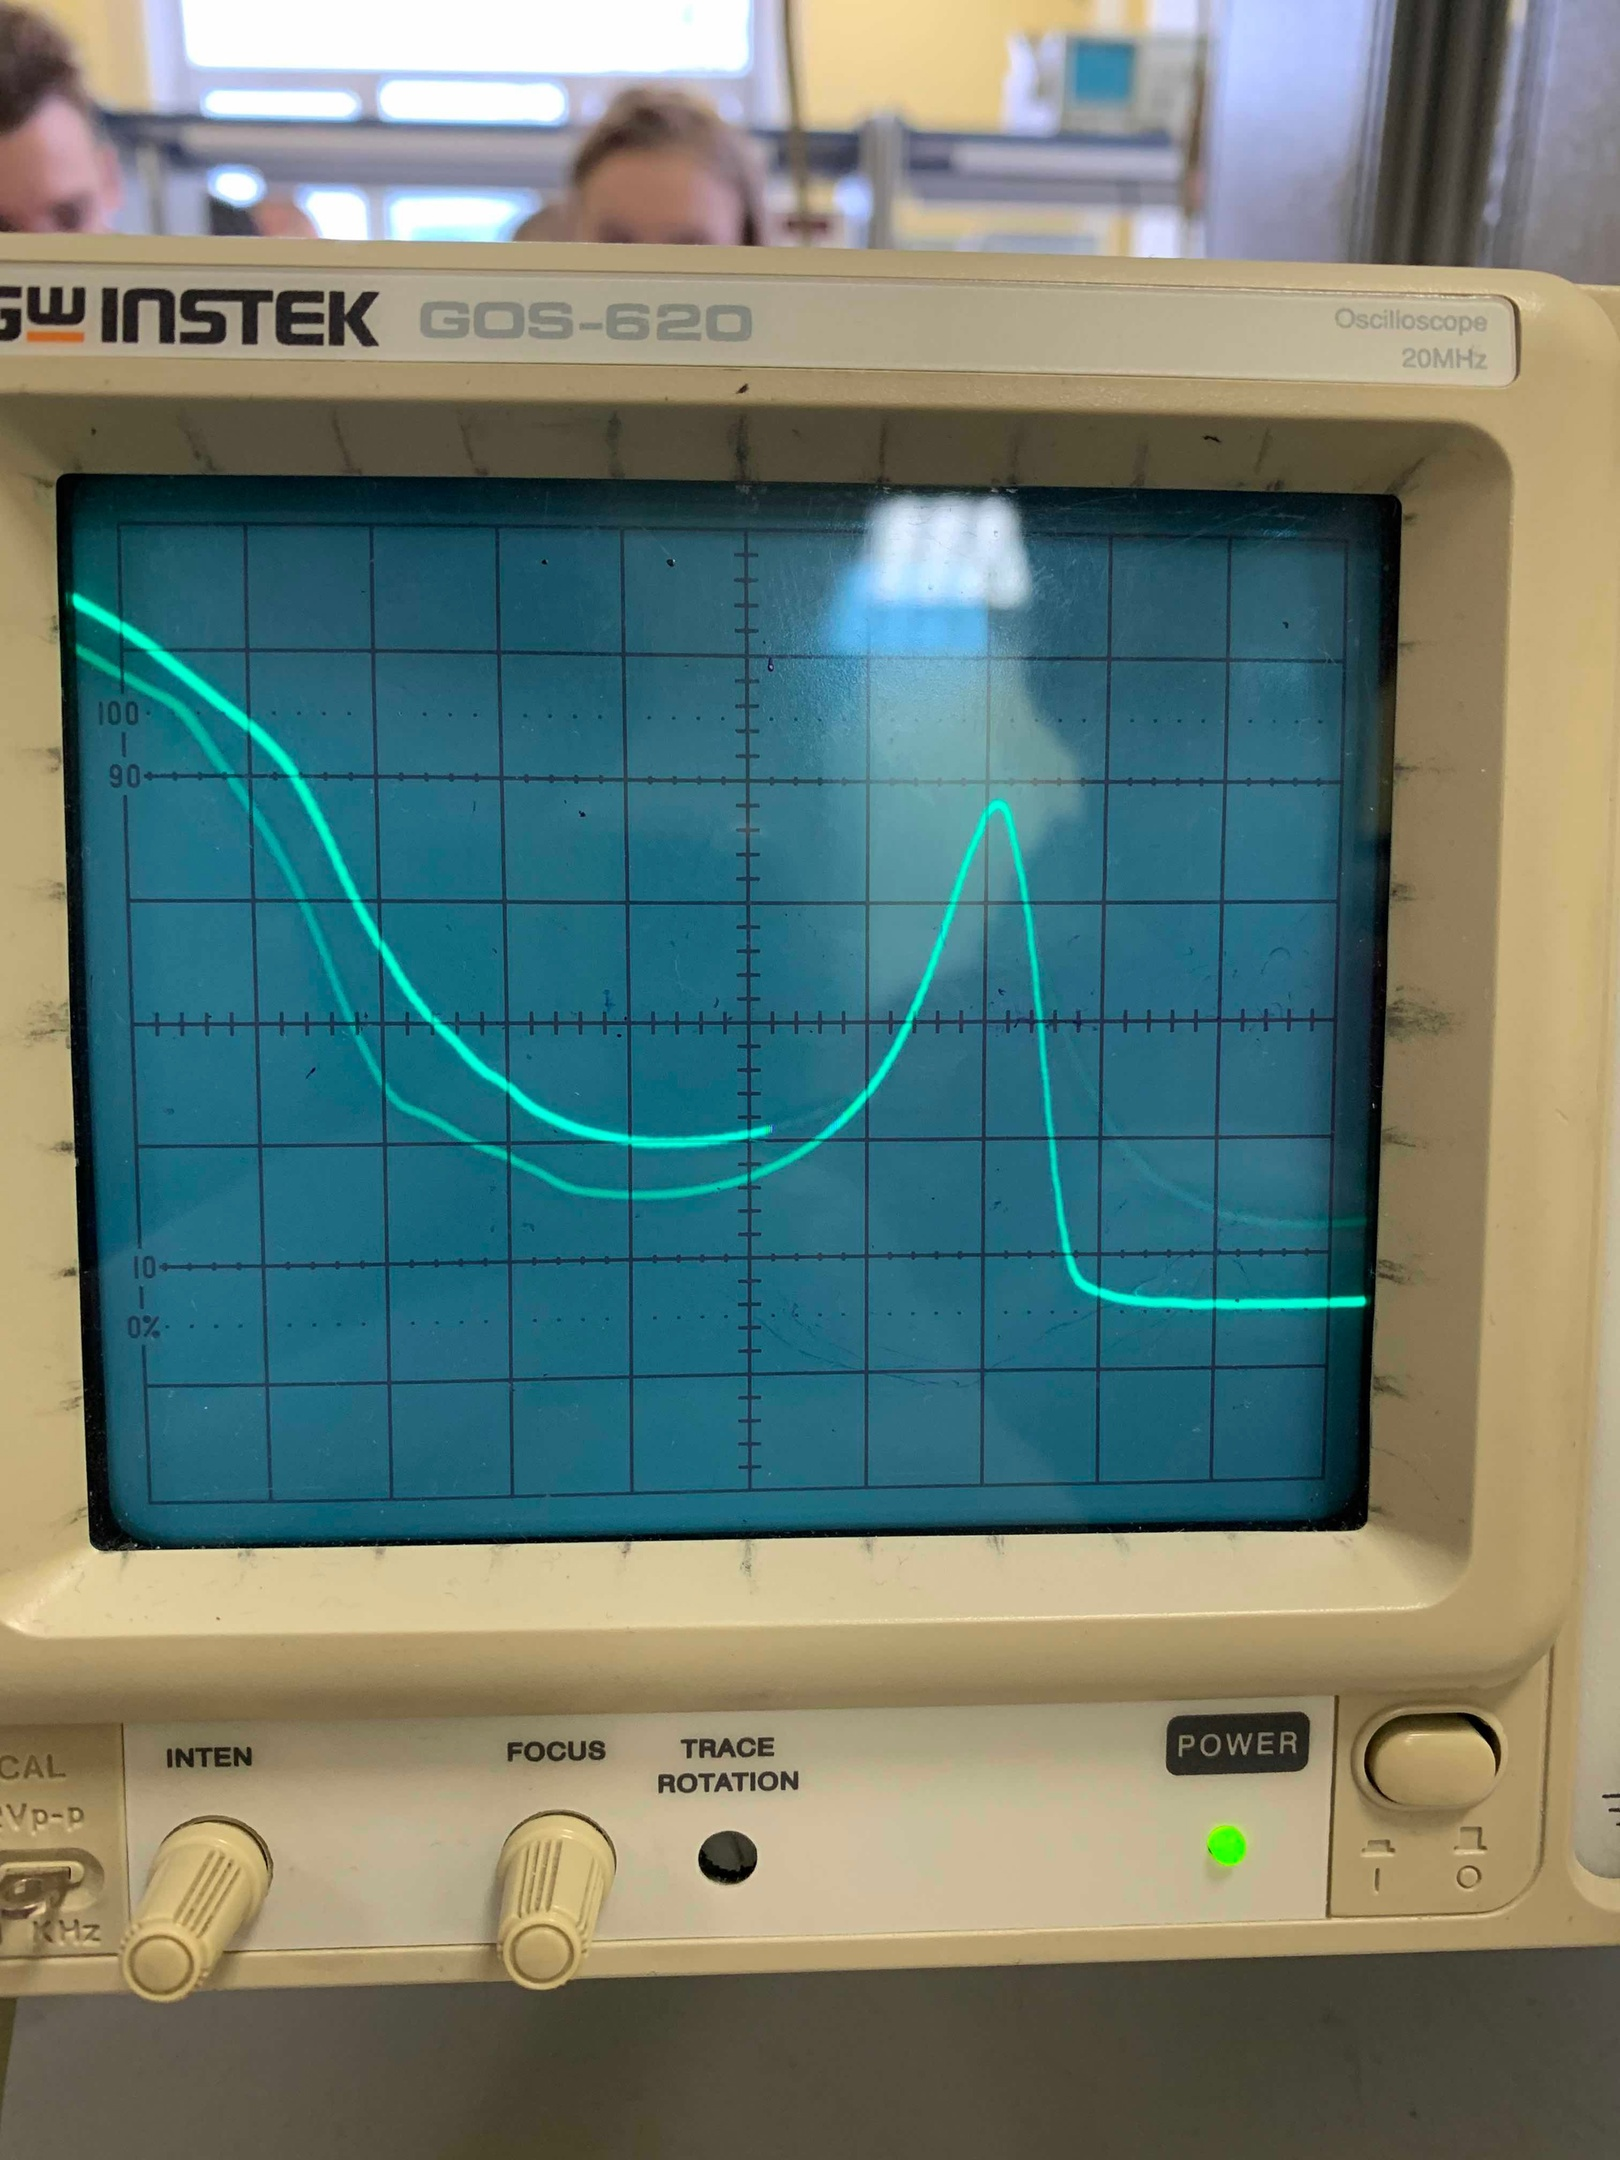
\includegraphics[scale=0.13]{Фото_2.PNG}
		\caption{$V_{\text{нак}} = 2.89$ В}
	\end{figure}

\item При поднесении к лампе постоянного магнита наблюдаются изменения в ВАХ на осциллографе,  вызванные тем,  что магнитное поле <<обостряет>> эффект Рамзауэра,  так как оно отклоняет любой электрон,  испытавший упругое столкновение.  Убедимся,  что влияние зависит от ориентации магнита относительно оси тиратрона.

\item Геометрические размеры тиратрона таковы, что напряжение пробоя практически совпадает с потенциалом ионизации.  Поэтому по результатам измерений напряжения пробоя можно определить,  каким газом наполнен тиратрон. 

	Рассчитаем размер электронной оболочки атома инертного газа,  эффективную глубину потенциальной ямы и потенциал ионизации газа:
	
	\begin{figure}[h!]
		\centering
		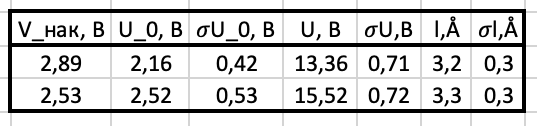
\includegraphics[scale=1]{Таблица_2.PNG}
	\end{figure}	

	При усреднении получаем: 
	
\[U_0 = (2,34 \pm 0,45) \text{ эВ} \]

\[ U = (14,44 \pm 0,72) \text{ эВ} \]

\[ l = (3,2 \pm 0,3) \text{ \AA } \]

$E_{\text{пр}} = (12,2 \pm 0,4)$ эВ,  что соответствует энергии ионизации ксенона.

\end{enumerate}

\textbf{Вольт-амперная характеристика в статическом режиме}

\begin{enumerate}

\item Проведем измерение ВАХ тиратрона:

	\begin{figure}[h!]
		\centering
		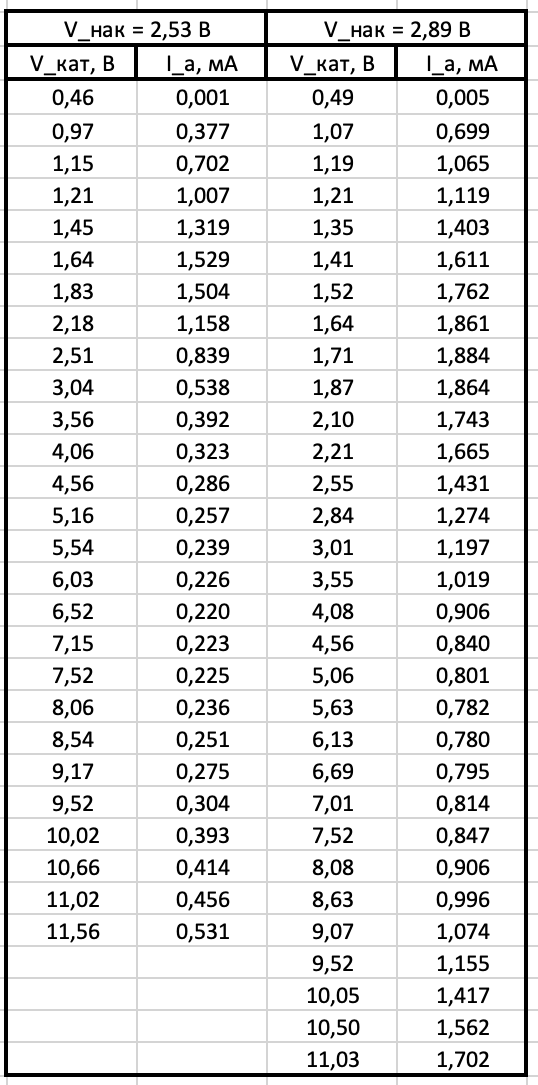
\includegraphics[scale=0.52]{Таблица_3.PNG}
	\end{figure}	

\newpage

\item По таблице построим график зависимости $I_{\text{анод}} = f(V_{\text{кат}})$.

	\begin{figure}[h!]
		\centering
		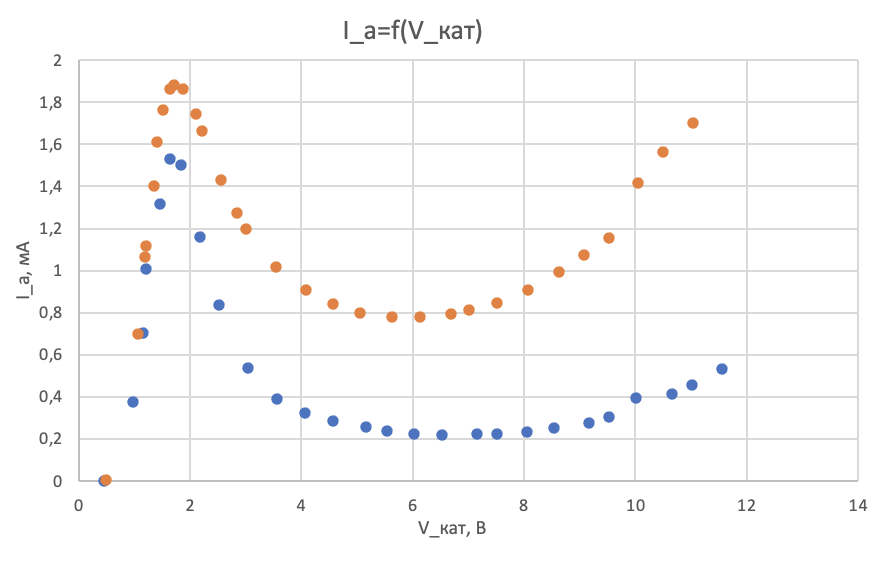
\includegraphics[scale=0.8]{График_2.PNG}
		\caption{синий -- $V_{\text{нак}} = 2.886$ В,  оранжевый -- $V_{\text{нак}} = 2.89$ В}
	\end{figure}

\item По полученному графику получим напряжения между катодом и сеткой, соответствующие первому максимуму и минимуму анодного тока:

	\begin{figure}[h!]
		\centering
		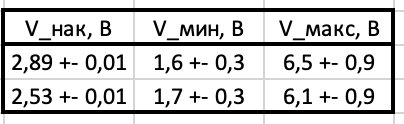
\includegraphics[scale=0.8]{Таблица_4.PNG}
	\end{figure}	


\item Проведем аналогичные расчеты для глубины потенциальной ямы и эффективного размера атома:

\[ U_0 = (2,04 \pm 0,52) \text{ В} \]

\[ l = (3,1 \pm 0,3) \text{ \AA } \]

Как мы видим, полученные данные согласуются с теми, что были полученны с помощью осциллографа в пределах погрешностей.

\item Оценим,  используя формулу

 \[k_2 l = \sqrt{\frac{2m(E_n + U_0)}{\hbar^2}}l = n \pi,\]
 
при каких напряжениях должны появляться максимумы в коэффициенте прохождения электронов для $n = 2, 3$.  Для этого выразим энергию $E_n$ через $E_1$:

\[E_n = n^2(E_1 + U_0) - U_0\]

Тогда получим:

\[E_2 = (20.1 \pm 3.4) \text{ эВ}\]

\[E_3 = (47.3 \pm 7.6) \text{ эВ}\]

\item Построим график зависимости $\omega = f(v_\text{кат})$ (с точностью до константы):

	\begin{figure}[h!]
		\centering
		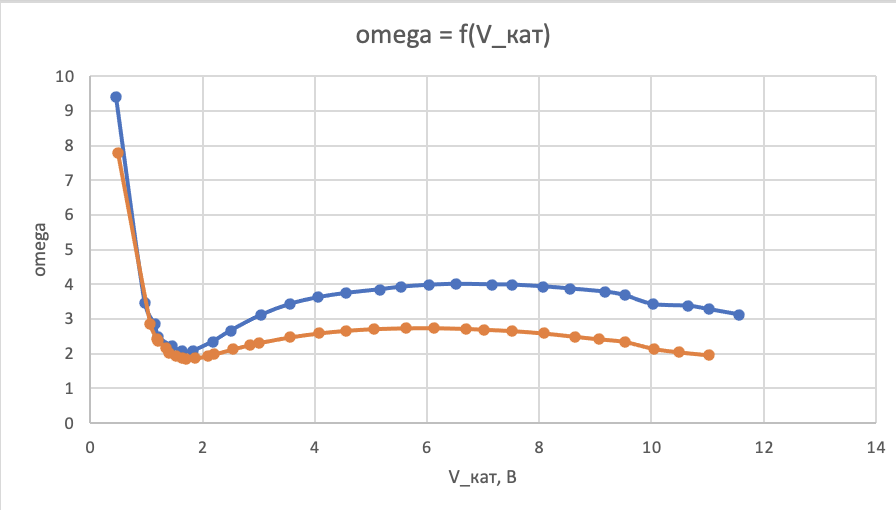
\includegraphics[scale=0.8]{График_3.PNG}
		\caption{синий -- $V_{\text{нак}} = 2.886$ В,  оранжевый -- $V_{\text{нак}} = 2.89$ В}
	\end{figure}

\end{enumerate}

\textbf{Вывод:}\\\par

\begin{enumerate}

\item Наблюдали ВАХ тиратрона в динамическом режиме при различных напряжениях накала, причем по напряжению пробоя определили, что используемый в эксперименте инертный газ - ксенон,  так как энергия ионизации ксенона -- 12.1 эВ,  а $E_\text{пр} = (12,2 \pm 0,4)$ эВ. 

\item Вычислили размер электронной оболочки атома ксенона $l_{\text{д}} = (3,2 \pm 0,3)  \text{ \AA}$, $l_{\text{с}} = (3,1 \pm 0,3)  \text{ \AA}$,  который близок к табличному значению $l_\text{табл} = 2,8 \text{ \AA}$. 

\item Вычислили эффективную глубину потенциальной ямы ксенона $U_{0\text{д}} = (2,34 \pm 0,45)$ эВ,  $U_{0\text{c}} = (2,04 \pm 0,52)$ эВ.

\item Динамический и статический способы измерения дают сравнительно хорошую точность и не сильно отличаются по результатам.

\item В ходе работы были получены графики зависимости $I_{\text{анод}}$ от $f(V_{\text{кат}})$ и $\omega$ от $f(V_{\text{кат}})$,  которые по форме совпадают с теоритическими.

\item Нашли энергии,  соответствующие максимумам на ВАХ для $n = 2 : E_2 = (20.1 \pm 3.4) \text{ эВ}$ и $n = 3 : E_3 = (47.3 \pm 7.6) \text{ эВ}$. 

\end{enumerate}

\end{document}